\chapter{Guide d'onda} 

\begin{figure}[h]
    \centering
    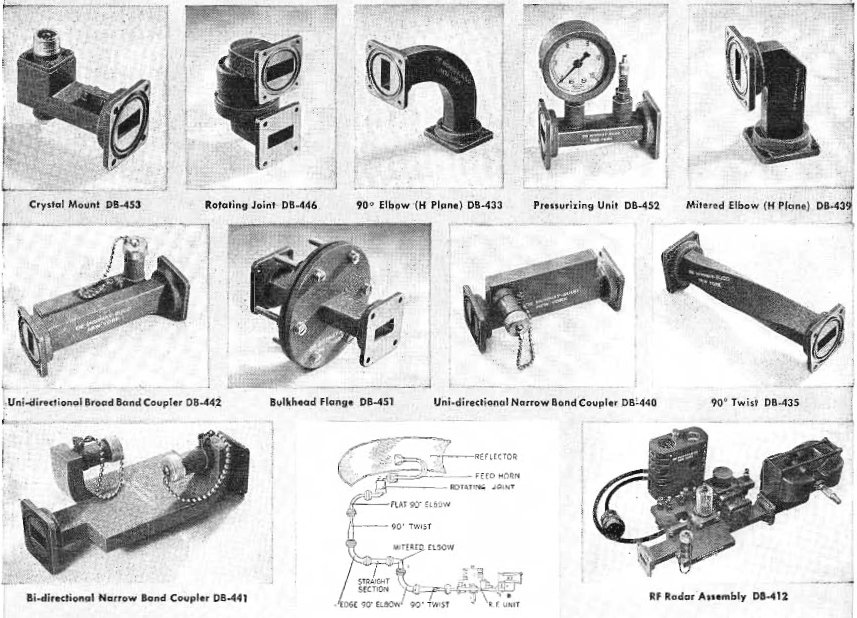
\includegraphics[scale = 0.5]{Waveguide_collection.jpg}
\end{figure} 

\newpage 

\section{Cosa sono le guide d'onda} 

\footnote{FWC - pag 395 \\ 8.1 Introduction}

La guida d'onda è una struttura, o parte di una struttura, che permette 
ad un'onda di propagarsi in una precisa direzione. \\ 

Se la guida d'onda cambia direzione, l'onda è costretta a seguirla. \\ 

I componenti trasversali dell'onda si propagheranno lungo la direzione di propagazione. \\ 

Generalmente, nelle analisi delle guide d'onda, siamo interessati alla distribuzione dei campi EM; 
ma, la cosa più importante è la dipendenza della costante di propagazione rispetto alla frequenza. \\ 

Dalla costante di propagazione è possibile calcolare la velocità dell'onda, 
la variazione di fase e l'attenuazione lungo la guida d'onda. \\ 

\newpage 

\section{Equazioni delle guide d'onda per sistemi uniformi} 
\footnote{FWC - pag 396 \\ 8.2 Basic equations and wave types for uniform systems}

Nelle guide d'onda considereremo onde del tipo: 

{\Large 
    \begin{equation}
        e^{\jmath \omega t - \gamma z}
    \end{equation}
}

quindi onde a tempo armonico $\jmath \omega t$ e che variano con la distanza $ - \gamma z$. \\ \\ 


\begin{tcolorbox}
    $\gamma$ dall'alfabeto greco si legge gamma 
\end{tcolorbox}


La costante di propagazione $\gamma$ sarà importante per le proprietà dell'onda, 
come ad esempio di quanto si attenua l'onda, la fase e la velocità di gruppo. \\ \\ 

Assumiamo nessuna densità di carica in ingresso e considereremo i conduttori della guida d'onda soddisfino l'equazione: 

{
    \Large
    \begin{equation}
        \kappa^{2} = \omega^{2} \mu \varepsilon
    \end{equation}
} 

Le equazioni dell'onda, che si riducono alle equazioni di Helmholtz per i campi fasoriali, saranno: 

{
    \Large 
    \begin{equation}
        \begin{cases}
            \nabla ^{2} \vec{E} = - \kappa ^{2}  \vec{E} \\ 
            \nabla ^{2} \vec{H} = - \kappa ^{2}  \vec{H} \\    
        \end{cases}
    \end{equation}
}

Nelle coordinate cartesiane, $\nabla ^{2}$, chiamato anche operatore di Laplace, può essere suddiviso in due parti: 

{
    \Large 
    \begin{equation}
        \begin{split}
            \nabla ^{2} \vec{E} 
            &= \frac{\partial ^{2} \vec{E}}{\partial x ^{2}} + \frac{\partial ^{2} \vec{E}}{\partial y ^{2}} + \frac{\partial ^{2} \vec{E}}{\partial z ^{2}}
            \\
            &= \nabla_t ^{2} \vec{E} + \frac{\partial ^{2} \vec{E}}{\partial z^{2}}  
        \end{split}
    \end{equation}
} 

dove, $\nabla_t ^{2}$ lo definiamo come operatore di Laplace trasversale. \newline 

Assumendo la funzione di propagazione lungo l'asse x $e^{-\gamma z}$, possiamo scrivere: 

{
    \Large
    \begin{equation} 
        \frac{\partial ^{2} \vec{E}}{\partial z^{2}} = \gamma ^{2} \vec{E}
    \end{equation}
}

Uguagliando i due modi di esprimere $\nabla ^{2} \vec{E}$ e sostituendo il 
valore di $ \frac{\partial ^{2} \vec{E}}{\partial z^{2}}$, possiamo scrivere la seguente equazione: 

{
    \Large 
    \begin{equation}
        \begin{cases}
            \nabla ^{2} \vec{E} = - \kappa ^{2}  \vec{E} \\
            \nabla ^{2} \vec{E} = \nabla_t ^{2} \vec{E} + \frac{\partial ^{2} \vec{E}}{\partial z^{2}}
        \end{cases} 
        \Rightarrow
        - \kappa ^{2}  \vec{E} = \nabla_t ^{2} \vec{E} + \gamma ^{2} \vec{E}
    \end{equation}
}

Oppure, svolgendo diversi passi algebrici: 

{
    \Large
    \begin{equation}
        \begin{split}
            \nabla_t ^{2} \vec{E} 
            &= - \kappa ^{2}  \vec{E} - \gamma ^{2}  \vec{E} \\ 
            &= -(\kappa ^{2} + \gamma ^{2}) \vec{E} 
        \end{split}
    \end{equation}
}

I passaggi algebrici svolti per $\nabla_t ^{2} \vec{E}$ possono essere svolti 
anche per $\nabla_t ^{2} \vec{H}$: 

{
    \Large
    \begin{equation}
        \nabla_t ^{2} \vec{H} = -(\kappa ^{2} + \gamma ^{2}) \vec{H}
    \end{equation}
}

$\nabla_t ^{2} \vec{E}$ e $\nabla_t ^{2} \vec{H}$ sono equazioni differenziali che devono essere soddisfatte 
nelle regione del dielettrico della linea di trasmissione o della guida d'onda. \\ 


La procedura standard è quella di trovare i componenti di $\vec{E}$ e $\vec{H}$ lungo 
l'asse z che soddisfano $\nabla_t ^{2} \vec{E}$ e $\nabla_t ^{2} \vec{H}$, quindi le condizioni al contorno, oppure 
esplicitato in una maniera differente, troviamo $E_z$ e $H_z$ in modo tale che siano le variabili indipendenti del sistema. \\ 

Consideriamo le equazioni di $e^{\jmath \omega t - \gamma z}$ 
in forma fasoriale divise nei loro componenti. \\ 

Dalle leggi di Maxwell avremo: 

{
    \Large 
    \begin{equation}
            \nabla \times \vec{E} 
            = \operatorname{rot}
            \begin{vmatrix}
                \hat{x} & \hat{y} &\hat{z} \\ \\ 
                \frac{\partial}{\partial x} & \frac{\partial}{\partial y} & -\gamma \\ \\ 
                E_x & E_y & E_z
            \end{vmatrix}  
    \end{equation}
}

Svolgendo diversi passi algebrici: 

{
    \Large 
    \begin{equation}
        \nabla \times \vec{E} 
            = 
            \hat{x} 
            \begin{vmatrix}
            \frac{\partial}{\partial y} & -\gamma \\  \\ 
            E_y & E_z 
            \end{vmatrix}
            -\hat{y} 
            \begin{vmatrix}
            \frac{\partial}{\partial x} & -\gamma \\  \\ 
            E_x & E_z 
            \end{vmatrix}
            +\hat{z} 
            \begin{vmatrix}
            \frac{\partial}{\partial x} & \frac{\partial}{\partial y} \\  \\ 
            E_x & E_y 
            \end{vmatrix}
    \end{equation}
}

{
    \Large 
    \begin{equation}
            \nabla \times \vec{E}
            = 
            \hat{x} 
            [
                \frac{\partial E_z}{\partial y} 
                +\gamma E_y
            ]    
            -\hat{y} 
            [
                \frac{\partial E_z}{\partial x} 
                +\gamma E_x
            ]    
            +\hat{z} 
            [
                \frac{\partial E_y}{\partial x} 
                + \frac{\partial E_x}{\partial y}
            ] 
    \end{equation}
}

{
    \Large 
    \begin{equation}
            \nabla \times \vec{E}
            =        
\hat{x} 
[
    \frac{\partial E_z}{\partial y} 
    +\gamma E_y
]    
+\hat{y} 
[
    -\frac{\partial E_z}{\partial x} 
    -\gamma E_x
]    
+\hat{z} 
[
    \frac{\partial E_y}{\partial x} 
    + \frac{\partial E_x}{\partial y}
] 
    \end{equation}
}       


Dalle equazioni di Maxwell in forma fasoriale: 

{
    \Large 
    \begin{equation}
        \nabla \times \vec{E} = -\jmath \omega \mu \vec{H}
    \end{equation}
}

Divendendo questa equazione nei vari assi cartesiani: \\ 

\textbf{Asse X} 

{
    \Large 
    \begin{equation}
        \frac{\partial E_z}{\partial y} + \gamma E_y 
        = 
        -\jmath \omega \mu H_x
    \end{equation}
}


\textbf{Asse Y} 

{
    \Large 
    \begin{equation}
        - \gamma E_x - \frac{\partial E_z}{\partial x}  
        = 
        -\jmath \omega \mu H_y
    \end{equation}
}



\textbf{Asse Z} 

{
    \Large 
    \begin{equation}
        \frac{\partial E_y}{\partial x} - \frac{\partial E_x}{\partial y} 
        = 
        -\jmath \omega \mu H_z
    \end{equation}
}

Sostituendo $\vec{H}$ ad $\vec{E}$, possiamo trovare le equazioni 
di Maxwell in forma fasoriale di: 

Dalle equazioni di Maxwell in forma fasoriale: 

{
    \Large 
    \begin{equation}
        \nabla \times \vec{H} = \jmath \omega \varepsilon \vec{E}
    \end{equation}
}


\textbf{Asse X} 

{
    \Large 
    \begin{equation}
        \frac{\partial H_z}{\partial y} + \gamma H_y 
        = 
        \jmath \omega \varepsilon E_x
    \end{equation}
}


\textbf{Asse Y} 

{
    \Large 
    \begin{equation}
        - \gamma H_x - \frac{\partial H_z}{\partial x}  
        = 
        \jmath \omega \varepsilon E_y
    \end{equation}
}



\textbf{Asse Z} 

{
    \Large 
    \begin{equation}
        \frac{\partial H_y}{\partial x} - \frac{\partial H_x}{\partial y} 
        = 
        \jmath \omega \varepsilon E_z
    \end{equation}
}

Ora è possibile trovare $E_x$, $E_y$, $H_x$, $H_y$ 
in funzione di $E_z$ e $H_z$. \\ 

I passaggi algebrici sono omessi, però basta sostituire i valori. \\ 

Alla fine troveremo i i valori di: 

{
    \Large 
    \begin{equation}
        \begin{cases}
            E_x = - \frac{1}{\gamma ^{2} + \kappa ^{2}} (\gamma \frac{\partial E_z}{\partial x} + \jmath \omega \mu \frac{\partial H_z}{\partial y}) \\ \\ 
            E_y =  \frac{1}{\gamma ^{2} + \kappa ^{2}} (- \gamma \frac{\partial E_z}{\partial y} + \jmath \omega \mu \frac{\partial H_z}{\partial x}) \\ \\ 
            H_x =  \frac{1}{\gamma ^{2} + \kappa ^{2}} (- \gamma \frac{\partial H_z}{\partial x} + \jmath \omega \varepsilon \frac{\partial E_z}{\partial y}) \\ \\ 
            H_y =  -\frac{1}{\gamma ^{2} + \kappa ^{2}} ( \gamma \frac{\partial H_z}{\partial y} + \jmath \omega \varepsilon \frac{\partial E_z}{\partial x}) 
        \end{cases}
    \end{equation}
}

È conveniente scrivere: 

{
    \Large
    \begin{equation}
        \begin{cases}
            \gamma = \jmath \beta \\ 
            \kappa_c ^{2} = \gamma^{2} + \kappa^{2} = \kappa^{2} - \beta^{2} 
        \end{cases}
    \end{equation}
}



Le equazioni precedentemente scritte, diventeranno: 

{
    \Large 
    \begin{equation}
        \begin{cases}
            E_x = - \frac{\jmath}{\kappa_c ^{2}} (\beta \frac{\partial E_z}{\partial x} + \omega \mu \frac{\partial H_z}{\partial y}) \\ \\ 
            E_y =  \frac{\jmath}{\kappa_c ^{2}} (- \beta \frac{\partial E_z}{\partial y} + \omega \mu \frac{\partial H_z}{\partial x}) \\ \\ 
            H_x =  \frac{\jmath}{\kappa_c ^{2}} (- \beta \frac{\partial H_z}{\partial x} + \omega \varepsilon \frac{\partial E_z}{\partial y}) \\ \\ 
            H_y =  -\frac{\jmath}{\kappa_c ^{2}} ( \beta \frac{\partial H_z}{\partial y} + \omega \varepsilon \frac{\partial E_z}{\partial x}) 
        \end{cases}
    \end{equation}
}

Inoltre possiamo scrivere: 

{
    \Large 
    \begin{equation}
        \begin{cases}
            \nabla_t ^{2} E_z = - \kappa_c ^{2} E_z \\ \\
            \nabla_t ^{2} H_z = - \kappa_c ^{2} H_z     
        \end{cases}
    \end{equation} 
}

\newpage